% =====================================================================
%  Conformal Risk Control for croco-clip detection — experiment report
%  Build:  pdflatex conformal_report.tex  (twice, for refs)
%  Figures: run  python docs/report/make_report_figures.py  first, to
%  (re)generate the cross-experiment comparison plots in ./figures/.
% =====================================================================
\documentclass[11pt,a4paper]{article}

\usepackage[margin=2.4cm]{geometry}
\usepackage{graphicx}
\usepackage{amsmath,amssymb}
\usepackage{booktabs}
\usepackage{siunitx}
\usepackage{xcolor}
\usepackage{caption}
\usepackage{subcaption}
\usepackage[hidelinks]{hyperref}
\usepackage{enumitem}

% Look for figures both in ./figures (generated comparisons) and in the
% per-experiment output folders (the runs' own diagnostic PNGs).
\graphicspath{{figures/}{../../outputs/}}

\newcommand{\lamhat}{\hat{\lambda}}
\newcommand{\code}[1]{\texttt{\small #1}}

\title{\textbf{Conformal Risk Control for Croco-Clip Detection}\\
       \large A unified calibration framework and an experimental study of
       losses, expansions, and sequential calibration}
\author{Yohan Le Morhedec}
\date{\today}

\begin{document}
\maketitle

\begin{abstract}
We wrap a trained YOLO croco-clip detector in a \emph{Conformal Risk Control}
(CRC) layer that turns the detector's raw boxes into prediction \emph{sets}
carrying a finite-sample, distribution-free guarantee: the expected value of a
user-chosen loss is provably bounded by a target level $\alpha$. This report
documents (i) the \code{Calibrator} architecture --- a single composable engine
parametrised by four pluggable components --- (ii) the two calibration
pipelines built on top of it (single-knob CRC and two-phase Sequential CRC),
(iii) the evaluation methodology, and (iv) a systematic experimental study
sweeping the loss definition, the expansion geometry, the calibrated knob, and
the sequential budget split. Every configuration is validated out of sample on
an $800$-image held-out test set, and all of them respect the guarantee. We
close with a prioritised roadmap and a list of targeted questions for a
conformal-prediction expert.
\end{abstract}

\tableofcontents

% =====================================================================
\section{Introduction and problem setting}
% =====================================================================
The detector locates ``croco'' rail clips in cropped orthophotos. A missed clip
is operationally expensive, so we do not want a point prediction --- we want a
\emph{prediction set} (a possibly enlarged set of boxes) that comes with a
guarantee on how often it fails to cover the true target. Conformal Risk Control
provides exactly this: given any monotone, bounded per-image loss
$L_i \in [0,1]$ and a calibration set of $n$ exchangeable images, it returns a
single scalar $\lamhat$ such that the expected test loss is bounded:
\begin{equation}
  \mathbb{E}\!\left[L(\lamhat)\right] \;\le\; \alpha .
  \label{eq:crc-guarantee}
\end{equation}
The whole study answers one practical question in many forms: \emph{what is the
cheapest way to spend the conformal margin so that the guarantee holds?}
``Cheapest'' is measured by an efficiency metric (mean box area or box count) ---
a guarantee that holds by predicting the whole image is useless.

% =====================================================================
\section{The CRC framework: the \texttt{Calibrator} architecture}
% =====================================================================
The core design decision is that \emph{one} calibration engine serves every
experiment in this report. Everything that differs between experiments is
injected as a pluggable component (file: \code{conformal/calibrator.py}).

\subsection{Four pluggable component types}
\begin{description}[leftmargin=1.4cm,style=nextline]
  \item[\code{PredictionFunction}] runs the detector on one image and returns a
    strict \code{[P,5]} tensor: pixel-space \code{xyxy} plus a confidence score
    in column~4, filtered at a confidence threshold. The score is carried
    end-to-end so confidence-aware components can read it.
  \item[\code{ExpansionFunction}] maps a raw prediction set to a conformal one,
    with signature \code{(set, $\lambda$, conf\_threshold)}. It must be
    \emph{monotone non-decreasing} in $\lambda$ so the risk is monotone
    non-increasing --- the precondition for the root search. The signature is
    wide enough to host geometric \emph{and} confidence-aware variants without
    touching the engine.
  \item[\code{LossFunction}] is the per-image failure metric
    $L_i(\text{set},\text{GT}) \in [0,1]$, monotone non-increasing in the
    expansion. \emph{This is where the user encodes ``what failure means.''}
  \item[\code{EfficiencyMetric}] is the per-image \emph{cost} (set size), kept
    orthogonal to the loss: the loss asks \emph{``is the GT covered?''}, the
    efficiency metric asks \emph{``how much did we predict to cover it?''}
\end{description}
The set-level \code{Risk} is just the mean of the per-image loss,
$\hat{R}_n = \tfrac1n\sum_i L_i$, so defining a new risk is literally
\code{Risk(other\_loss)}.

\subsection{The calibration rule}
\code{Calibrator.calibrate} caches one prediction pass over the calibration set
and then, for each candidate $\lambda$ probed by Brent's method, re-applies
\emph{only} the expansion (so cost stays at $N$ model calls). It returns
\begin{equation}
  \lamhat \;=\; \inf\Bigl\{\lambda :
   \underbrace{\tfrac{n}{n+1}\hat{R}_n(\lambda) + \tfrac{1}{n+1}}_{\text{finite-sample correction } \tilde R(\lambda)}
   \;\le\; \alpha \Bigr\}.
  \label{eq:crc-rule}
\end{equation}
The $+\tfrac{1}{n+1}$ term protects against one extra worst-case test sample and
vanishes as $n\to\infty$. A guard handles the step-function nature of the
discrete loss (nudging $\lamhat$ past a step where Brent lands on the wrong
side), and an explicit error is raised when images with zero surviving
predictions \emph{lock} the loss at $1.0$ and no $\lambda$ can satisfy the bound
(observed at $\alpha=0.085$, see \S\ref{sec:summary}).

\subsection{Evaluation: \texttt{EvaluationResult}}
\code{Calibrator.evaluate} is the out-of-sample counterpart. From a single
prediction pass it produces an \code{EvaluationResult} bundling: the test risk
vs.\ $\alpha$ (\code{coverage\_satisfied}, \code{slack}), the per-image loss
distribution (\code{n\_perfect}, \code{n\_locked}), the efficiency cost and
\code{inflation\_ratio}, an optional risk curve $\hat R(\lambda)$, and arbitrary
\code{extra} diagnostics (false-positive / true-positive counts). It is generic
in the CRC components, which is why the same object reports every experiment
below.

% =====================================================================
\section{The two pipelines}
% =====================================================================
\subsection{Single-knob CRC}
\code{scripts/crc\_common.py:run\_pipeline} is a thin shell: calibrate
$\lamhat$, evaluate on test with a $\lambda$-sweep, re-evaluate at a baseline
operating point, compare, and emit all plots + overlays + a \code{results.txt}.
Each experiment is then a $\sim$15-line CONFIG block selecting a loss, an
expansion, an efficiency metric, and a baseline. The baseline is whatever
$\lambda$ reproduces the model's normal operating point ($\lambda=0$ for
geometric expansions; $\lambda = 1-T_{\text{std}}$ for the confidence knob,
since $\lambda=0$ there is the empty set).

\subsection{Sequential CRC (SeqCRC)}
SeqCRC (\code{conformal/seqcrc.py}, \code{scripts/calibrate\_seqcrc.py})
controls two complementary failure modes with two reuses of the \emph{same}
\code{Calibrator}, under a Bonferroni split $\alpha = \alpha_{\text{cnf}} +
\alpha_{\text{loc}}$:
\begin{enumerate}[leftmargin=1.6cm]
  \item \textbf{Phase 1 (confidence).} Detection-miss loss + confidence-filter
    knob: lower the objectness threshold until $\le\alpha_{\text{cnf}}$ of
    frames have an \emph{undetected} target. Yields $\lambda_{\text{cnf}}$ and
    an effective threshold $T_{\text{eff}} = \max(\text{floor},\,1-\lambda_{\text{cnf}})$.
  \item \textbf{Phase 2 (localization).} On the \emph{survivor} frames only
    (target detected at $T_{\text{eff}}$), grow boxes with an additive pixel
    margin under the $75\%$-coverage loss until $\le\alpha_{\text{loc}}$ of
    survivors fall short. Yields $\lambda_{\text{loc}}$.
\end{enumerate}
Because the two failure events partition the end-to-end failure
($\{\text{final coverage}<75\%\}\subseteq\{\text{target missed}\}\cup\{\text{detected but}<75\%\}$),
the union bound certifies the global $\alpha$. The honest validator is the
end-to-end empirical risk on the full test set.

\paragraph{Top-1 prediction selection.} SeqCRC additionally wraps the detector in
a \code{TopKPredictor} ($K=1$, file \code{conformal/prediction/top1.py}): only the
single highest-confidence box per frame is kept. This is a deliberate choice for
the single-object regime --- each cropped frame contains at most one croco clip.
Phase~1 drives the objectness threshold down toward the floor ($0.001$) to recover
missed targets; without top-1 selection that low threshold would flood every frame
with spurious low-confidence boxes, inflating the prediction-set area in Phase~2
and degrading precision. Keeping the top box turns ``lower the threshold'' into
``trust the detector's best guess for the one object,'' so the recovered detections
are the right ones rather than a swarm of false positives. The price is a feasibility
constraint: with $K=1$, Phase~1 can only meet $\alpha_{\text{cnf}}$ if that budget
exceeds the irreducible rate at which the top-1 box is \emph{not} the target (i.e.\
the highest-confidence box is a false positive); \code{scripts/diagnose\_top1.py}
measures that rate to confirm the chosen $\alpha_{\text{cnf}}$ is admissible. The
single-knob CRC experiments (\S5.1--5.3) keep all boxes, since they never lower the
threshold; top-1 is specific to SeqCRC's Phase~1. Top-1 selection was a refinement
added after the first SeqCRC run: the headline $50/50$ run (\code{seqcrc\_09}) keeps
all boxes, while the budget-split sweep in \S\ref{sec:seqcrc} uses top-1 --- as the
near-identical risks show, top-1 mainly buys precision and a smaller prediction set,
not lower risk.

% =====================================================================
\section{Evaluation methodology}
% =====================================================================
Every run uses a fixed $800$-image calibration split and a disjoint $800$-image
test split. We read three things off each run:
\begin{enumerate}[leftmargin=1.6cm,nosep]
  \item \textbf{Validity} --- does test risk $\le\alpha$ hold out of sample?
    (the guarantee is in expectation, so we expect, but cannot demand, this on
    every finite draw).
  \item \textbf{Efficiency} --- the inflation ratio and mean set size: the price
    paid for validity.
  \item \textbf{Generalisation} --- calibration risk vs.\ test risk at $\lamhat$,
    to expose any over-fit of the calibration set.
\end{enumerate}
Per-run diagnostics are emitted automatically: \code{risk\_curve.png},
\code{loss\_histogram.png}, \code{efficiency\_cost.png},
\code{calib\_vs\_test.png}, \code{with\_vs\_without.png}, and zoomed
WITHOUT-vs-WITH overlays on the images calibration helped most.

% =====================================================================
\section{Experiments}
% =====================================================================
All experiments use $\alpha = 0.09$ unless stated; calibration and test are both
$n=800$.

% ---------------------------------------------------------------------
\subsection{Loss definition: pixel-wise recall vs.\ 75\% coverage-indicator}
% ---------------------------------------------------------------------
Holding the expansion fixed (multiplicative), we compare two loss philosophies:
\begin{itemize}[nosep]
  \item \textbf{Pixel-wise recall} ($\code{crc\_09}$): $L_i = 1 - \overline{\text{coverage}}$,
    a graded loss summing the fraction of each GT's pixels recovered.
  \item \textbf{75\% coverage-indicator} ($\code{crc\_cov\_09}$):
    $L_i = \tfrac1{n_i}\sum_k \mathbf{1}\{\text{coverage}(GT_k)<0.75\}$,
    a binary ``found / missed'' notion at a 75\% bar.
\end{itemize}

\begin{table}[h]\centering
\caption{Loss definition (multiplicative expansion, $\alpha=0.09$).}
\begin{tabular}{lccccc}
\toprule
Loss & $\lamhat$ & test risk & raw risk & inflation & fully missed \\
\midrule
Pixel-wise recall      & 0.289 & 0.0798 & 0.1045 & $2.49\times$ & 62/800 \\
75\% coverage-indicator& 0.237 & 0.0775 & 0.1175 & $2.17\times$ & 62/800 \\
\bottomrule
\end{tabular}
\end{table}

The graded pixel loss is harder to satisfy (larger $\lamhat$, more inflation)
because it charges partial misses continuously; the binary 75\% loss saturates
once a GT clears the bar, so it stops growing boxes sooner. The coverage loss is
the better operational fit for ``a clip is either found or not'' and is the loss
of record for the remaining experiments.

\begin{figure}[h]\centering
  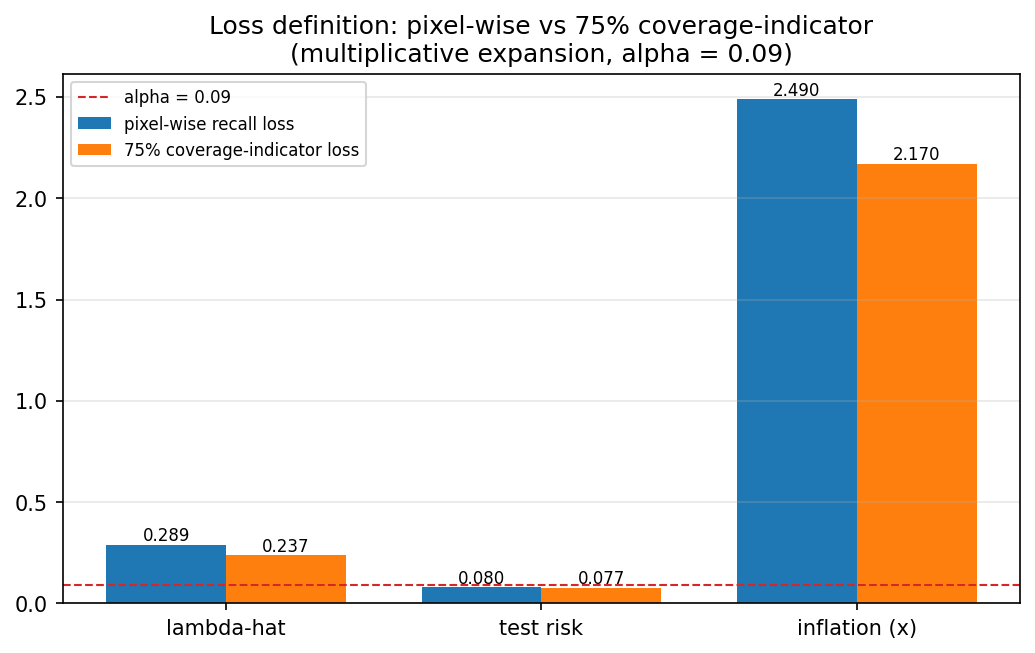
\includegraphics[width=0.62\textwidth]{fig_loss_comparison.png}
  \caption{Pixel-wise vs.\ 75\% coverage-indicator loss: calibrated margin,
  test risk, and inflation. \emph{Plot to underline:} the loss choice changes
  the \emph{cost} of the guarantee, not its validity.}
\end{figure}

\textbf{Supporting per-run figures:} \code{crc\_09/risk\_curve.png} (graded loss
decays smoothly) vs.\ \code{crc\_cov\_09/risk\_curve.png} (binary loss is a step
that flattens immediately past $\lamhat$); their \code{loss\_histogram.png}
side by side.

% ---------------------------------------------------------------------
\subsection{Expansion geometry: multiplicative, asymmetric, additive}
% ---------------------------------------------------------------------
Holding the loss fixed (75\% coverage), we compare three geometric expansions.
All three reach essentially the same risk; they differ in \emph{how much area}
they spend to get there --- the central efficiency result.

\begin{table}[h]\centering
\caption{Expansion geometry (75\% coverage loss, $\alpha=0.09$).
Raw mean box area $=85$\,px$^2$ in every case.}
\begin{tabular}{lcccc}
\toprule
Expansion & $\lamhat$ & test risk & mean area (px$^2$) & inflation \\
\midrule
Multiplicative ($w\lambda,h\lambda$)              & 0.237 & 0.0775 & 186 & $2.17\times$ \\
Asymmetric ($\tfrac{w\lambda}{3},h\lambda$)       & 0.237 & 0.0775 & 162 & $1.89\times$ \\
Additive ($+\lambda$ px/side, $\lamhat=1.14$\,px) & 1.138 & 0.0788 & 131 & $1.54\times$ \\
\bottomrule
\end{tabular}
\end{table}

For these thin, small clips the \textbf{additive} margin is the most efficient
($1.54\times$): a fixed pixel pad covers localisation slack without scaling with
box size. The \textbf{asymmetric} variant beats the symmetric multiplicative by
shrinking lateral growth $3\times$ (lateral spill is wasteful for elongated
targets) while keeping vertical generosity.

\begin{figure}[h]\centering
  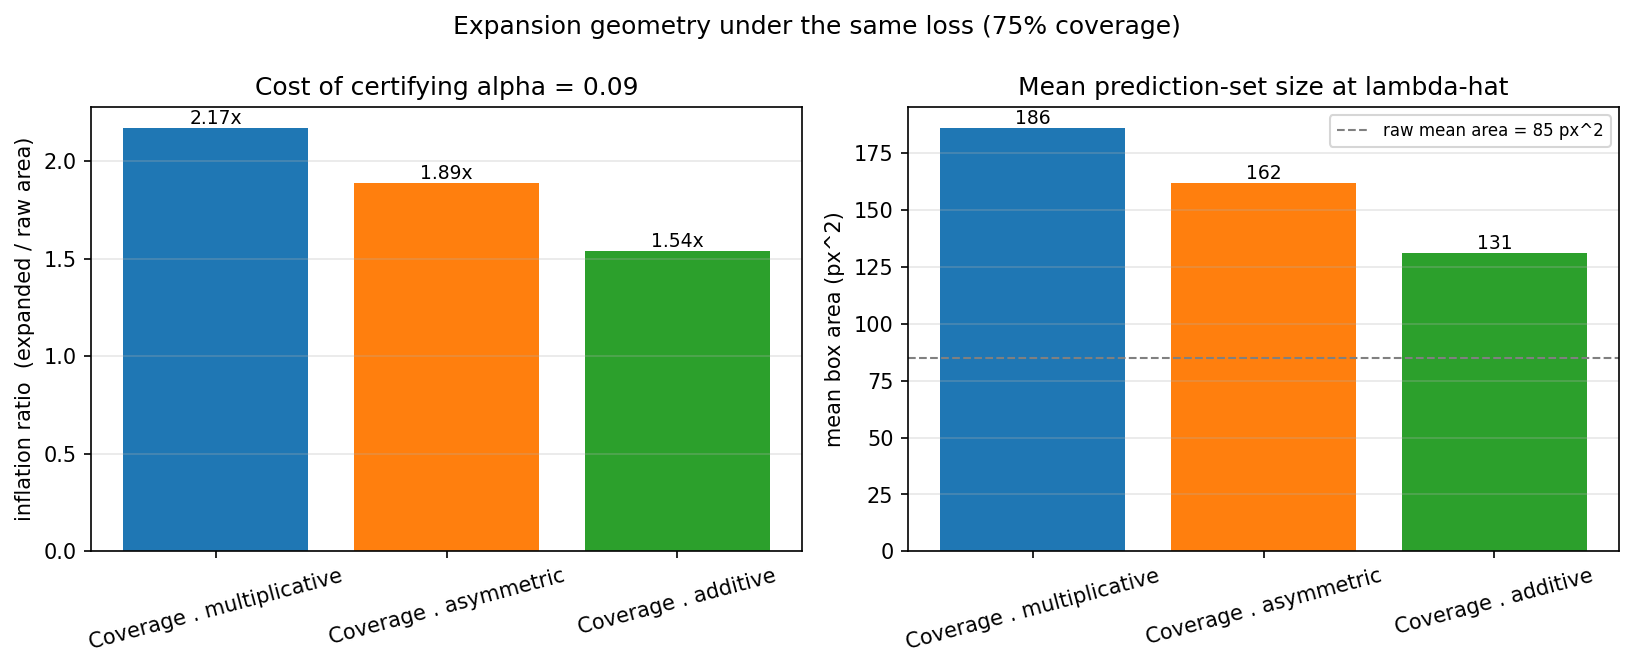
\includegraphics[width=0.92\textwidth]{fig_expansion_efficiency.png}
  \caption{\emph{Key plot.} Same guarantee, three geometries: inflation ratio
  (left) and mean prediction-set area (right). Additive is cheapest for this
  target shape.}
\end{figure}

\begin{figure}[h]\centering
  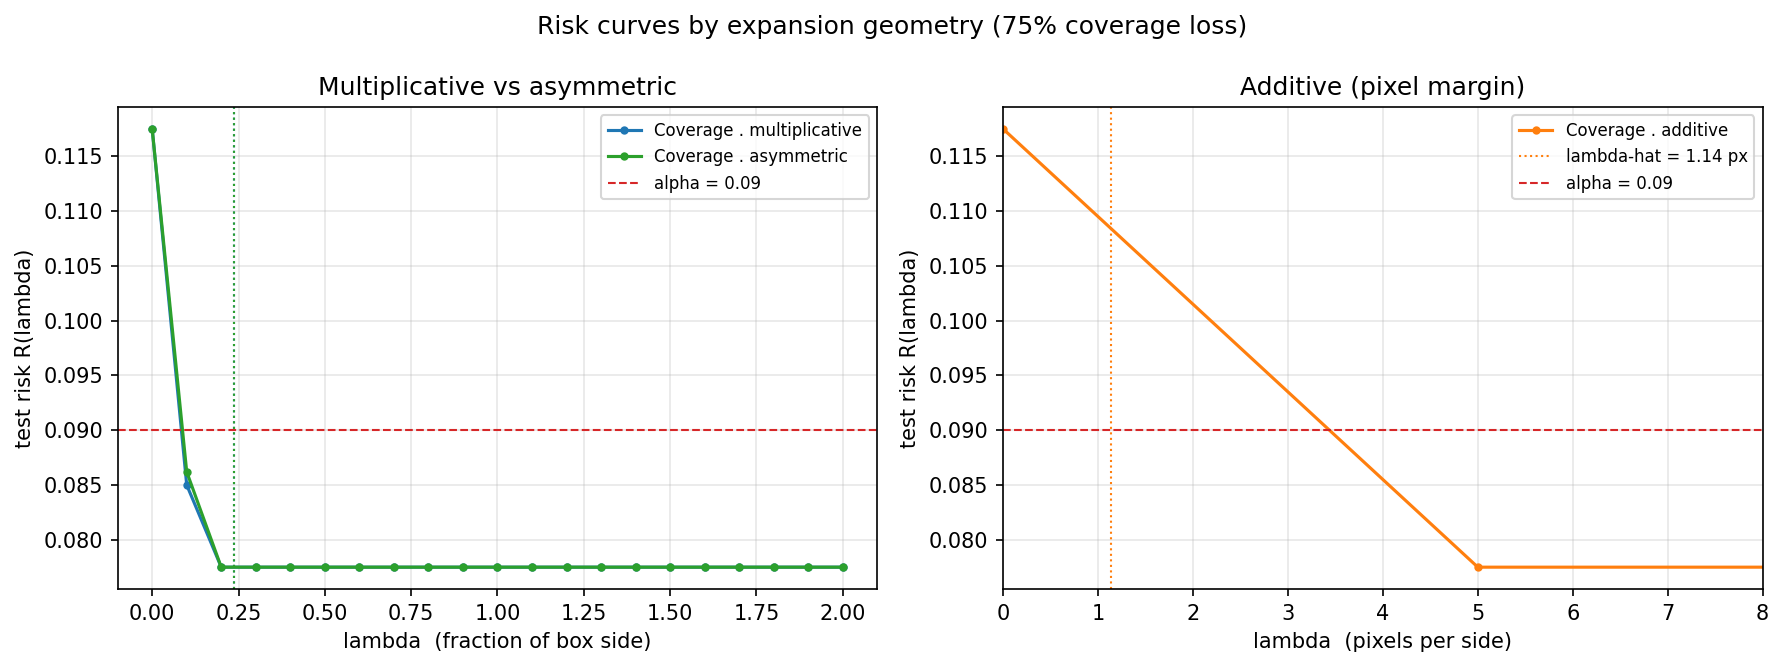
\includegraphics[width=0.92\textwidth]{fig_expansion_riskcurves.png}
  \caption{Risk curves $\hat R(\lambda)$ by geometry. Multiplicative/asymmetric
  share a dimensionless $\lambda$ (fraction of box side); additive's $\lambda$
  is in pixels, hence its own panel. All cross $\alpha$ and flatten, confirming
  monotonicity.}
\end{figure}

\textbf{Supporting per-run figures:} the \code{examples/example\_00.png}
overlays from \code{crc\_add\_cov\_09} vs.\ \code{crc\_asym\_cov\_09\_06} show
visually how each geometry pads the same clip.

% ---------------------------------------------------------------------
\subsection{Confidence-wise vs.\ box-size expansion}
% ---------------------------------------------------------------------
A different axis: instead of \emph{growing} existing boxes, the
confidence-filter knob \emph{admits more boxes} by lowering the objectness
threshold (\code{crc\_conf\_09}, $T_{\text{eff}}=0.251$). The two attack
different failure modes:

\begin{table}[h]\centering
\caption{Confidence-wise (admit boxes) vs.\ box-size (grow boxes), 75\% coverage,
$\alpha=0.09$.}
\begin{tabular}{lcccc}
\toprule
Expansion & $\lamhat$ & test risk & raw missed & calibrated missed \\
\midrule
Confidence-filter (threshold knob) & 0.749 & 0.0850 & 94/800 & 68/800 \\
Multiplicative (box size)          & 0.237 & 0.0775 & 94/800 & 62/800 \\
\bottomrule
\end{tabular}
\end{table}

Geometric expansion cannot help a frame with \emph{no} surviving box (an empty
set stays empty), so it relies on the detector having already fired. The
confidence knob recovers genuinely missed detections by admitting lower-score
boxes --- the mechanism SeqCRC's Phase~1 exploits. This is precisely the gap
SeqCRC is designed to close.

\begin{figure}[h]\centering
  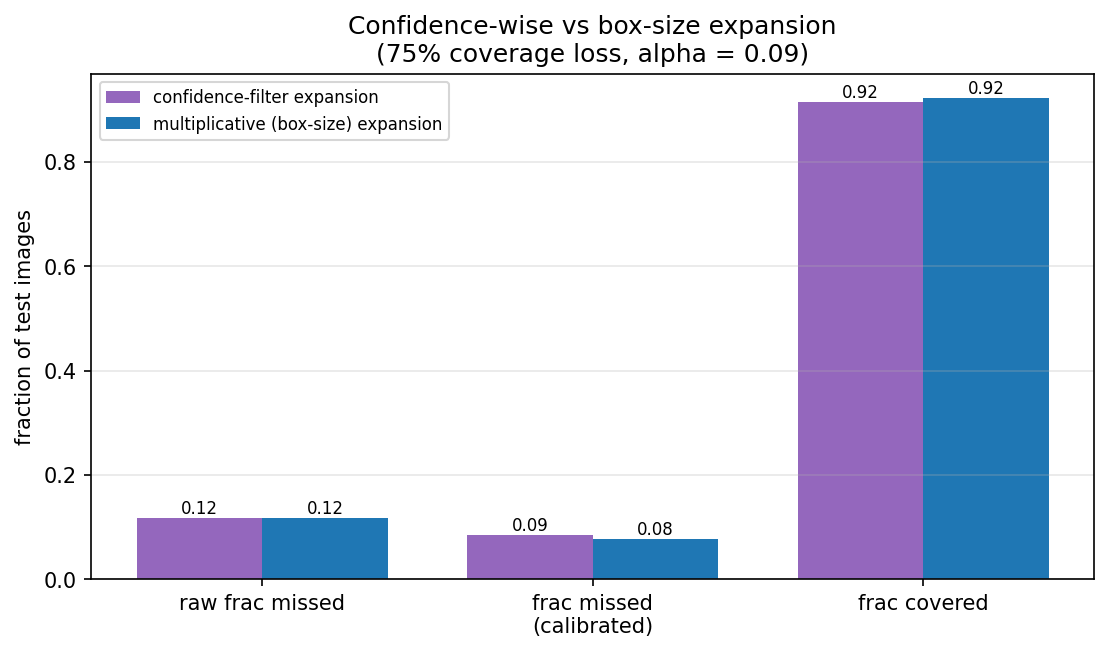
\includegraphics[width=0.6\textwidth]{fig_confidence_vs_geometric.png}
  \caption{\emph{Plot to underline:} two ways to spend $\lambda$ and their
  effect on the fully-missed fraction. Both certify $\alpha$, but only the
  confidence knob directly attacks missed detections.}
\end{figure}

\textbf{Supporting per-run figure:} \code{crc\_conf\_09/risk\_curve.png} shows
the risk staying flat until the threshold falls enough to admit boxes, then
dropping sharply --- the characteristic confidence-knob shape, very different
from the smooth geometric decay.

% ---------------------------------------------------------------------
\subsection{Sequential CRC and the budget split}
\label{sec:seqcrc}
% ---------------------------------------------------------------------
SeqCRC combines both mechanisms: Phase~1 (confidence) recovers detections,
Phase~2 (additive) localises them, under $\alpha=\alpha_{\text{cnf}}+\alpha_{\text{loc}}=0.09$.
The headline run (\code{seqcrc\_09}, 50/50 split) achieves an end-to-end test
risk of \textbf{0.040} --- roughly half of any single-knob method --- by
recovering many more clips (fully missed $94\to32$/800) at a tiny precision cost
($+1$ false-positive box on $800$ frames).

\begin{table}[h]\centering
\caption{SeqCRC under different union-bound splits (top-1 box per frame,
$\alpha=0.09$). The 50/50 row without top-1 selection (\code{seqcrc\_09}) gives
$T_{\text{eff}}{=}0.162$, $\lambda_{\text{loc}}{=}0.34$, e2e risk $0.040$.}
\begin{tabular}{lccccc}
\toprule
Split $\alpha_{\text{cnf}}/\alpha_{\text{loc}}$ & $\lambda_{\text{cnf}}$ & $T_{\text{eff}}$ & survivors $n_{\text{loc}}$ & $\lambda_{\text{loc}}$ (px) & e2e test risk \\
\midrule
35 / 65 & 0.901 & 0.099 & 222/800 & 0.438 & 0.0387 \\
50 / 50 & 0.839 & 0.162 & 211/800 & 0.548 & 0.0437 \\
75 / 25 & 0.742 & 0.258 & 193/800 & 1.138 & 0.0525 \\
\bottomrule
\end{tabular}
\end{table}

The split is a genuine knob. Giving \emph{more} budget to Phase~1 (35/65 column,
small $\alpha_{\text{cnf}}$ forces a tighter detection guarantee) drives
$T_{\text{eff}}$ down, admits more boxes, leaves Phase~2 an easier localisation
job (smaller $\lambda_{\text{loc}}$), and yields the lowest end-to-end risk here.
All splits pass with wide slack, so the union bound is conservative --- the
empirical risk sits far below $\alpha$.

\begin{figure}[h]\centering
  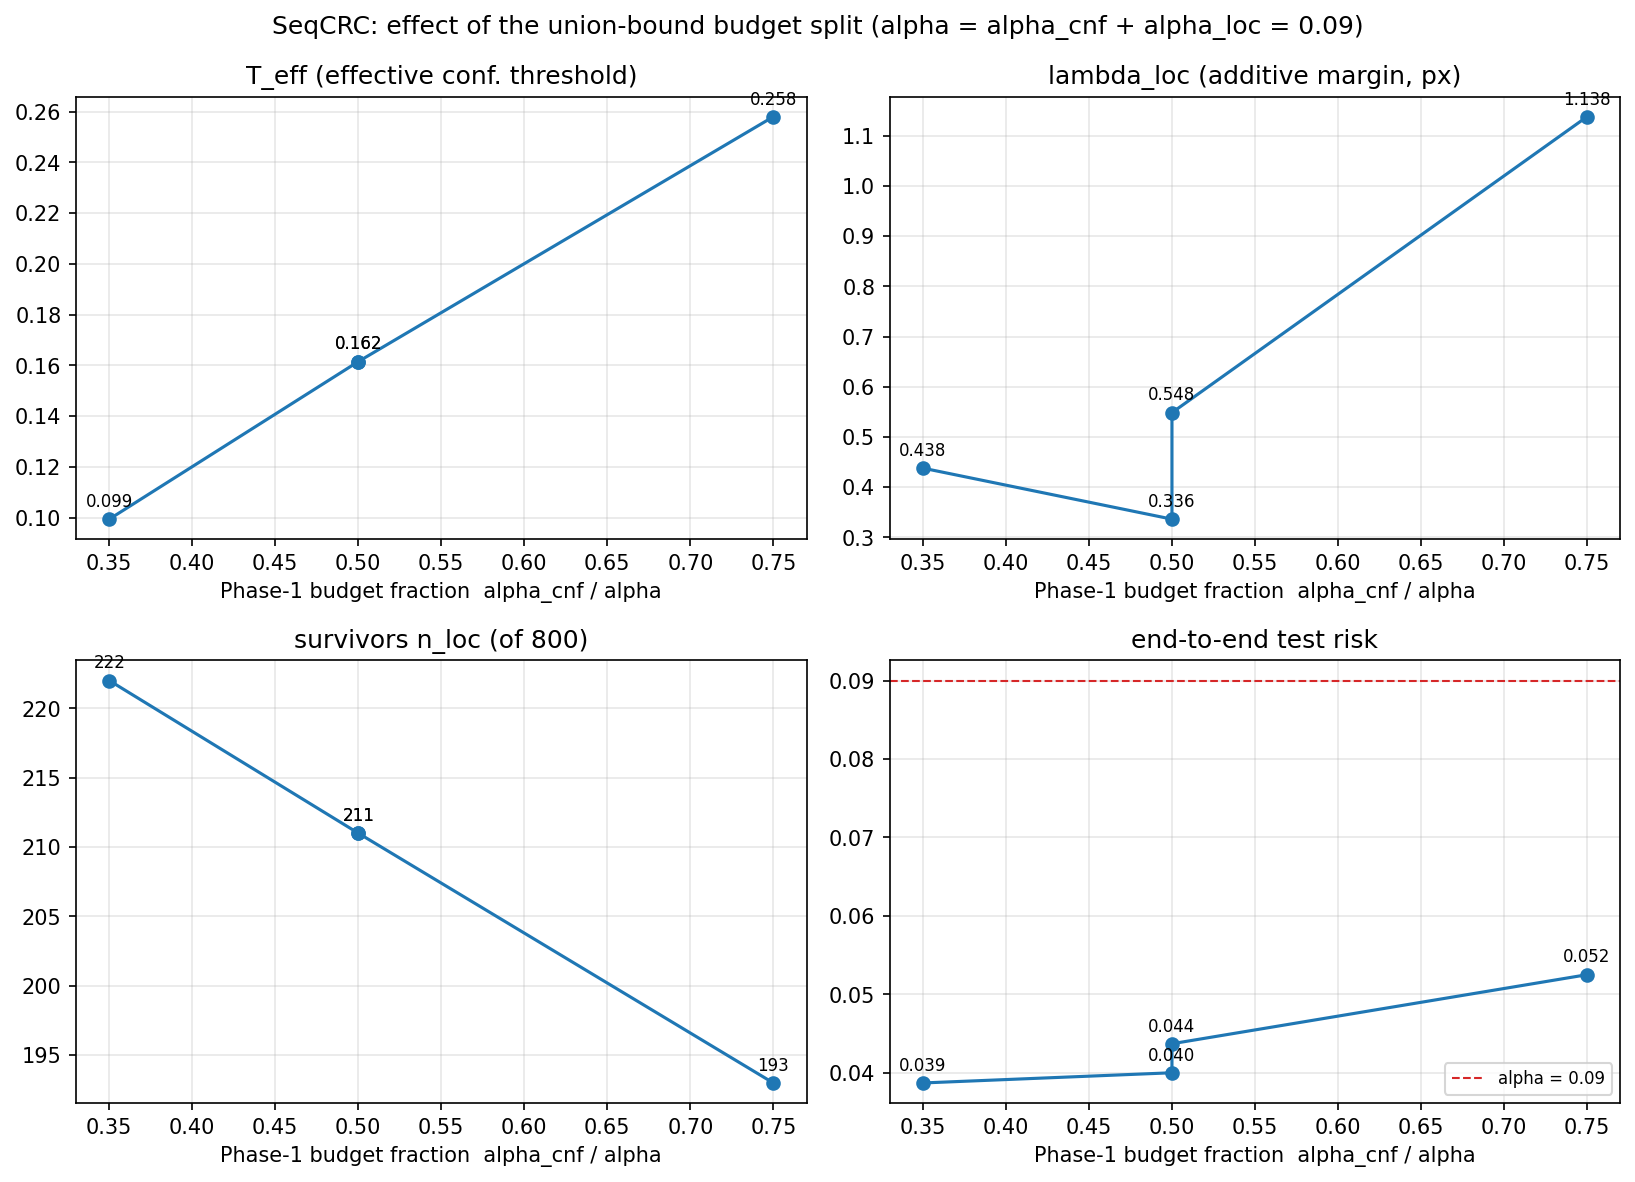
\includegraphics[width=0.95\textwidth]{fig_seqcrc_allocation.png}
  \caption{\emph{Key SeqCRC plot.} How the budget split moves each knob:
  $T_{\text{eff}}$, $\lambda_{\text{loc}}$, survivor count, and end-to-end test
  risk vs.\ the Phase-1 budget fraction.}
\end{figure}

\textbf{Supporting per-run figures:} \code{seqcrc\_09/with\_vs\_without.png}
(the large drop in fully-missed frames) and the Phase-2
\code{seqcrc\_09/examples/example\_00.png} overlays (filtered-but-unexpanded vs.\
$+\lambda_{\text{loc}}$).

% =====================================================================
\section{Cross-method summary}
\label{sec:summary}
% =====================================================================
\begin{figure}[h]\centering
  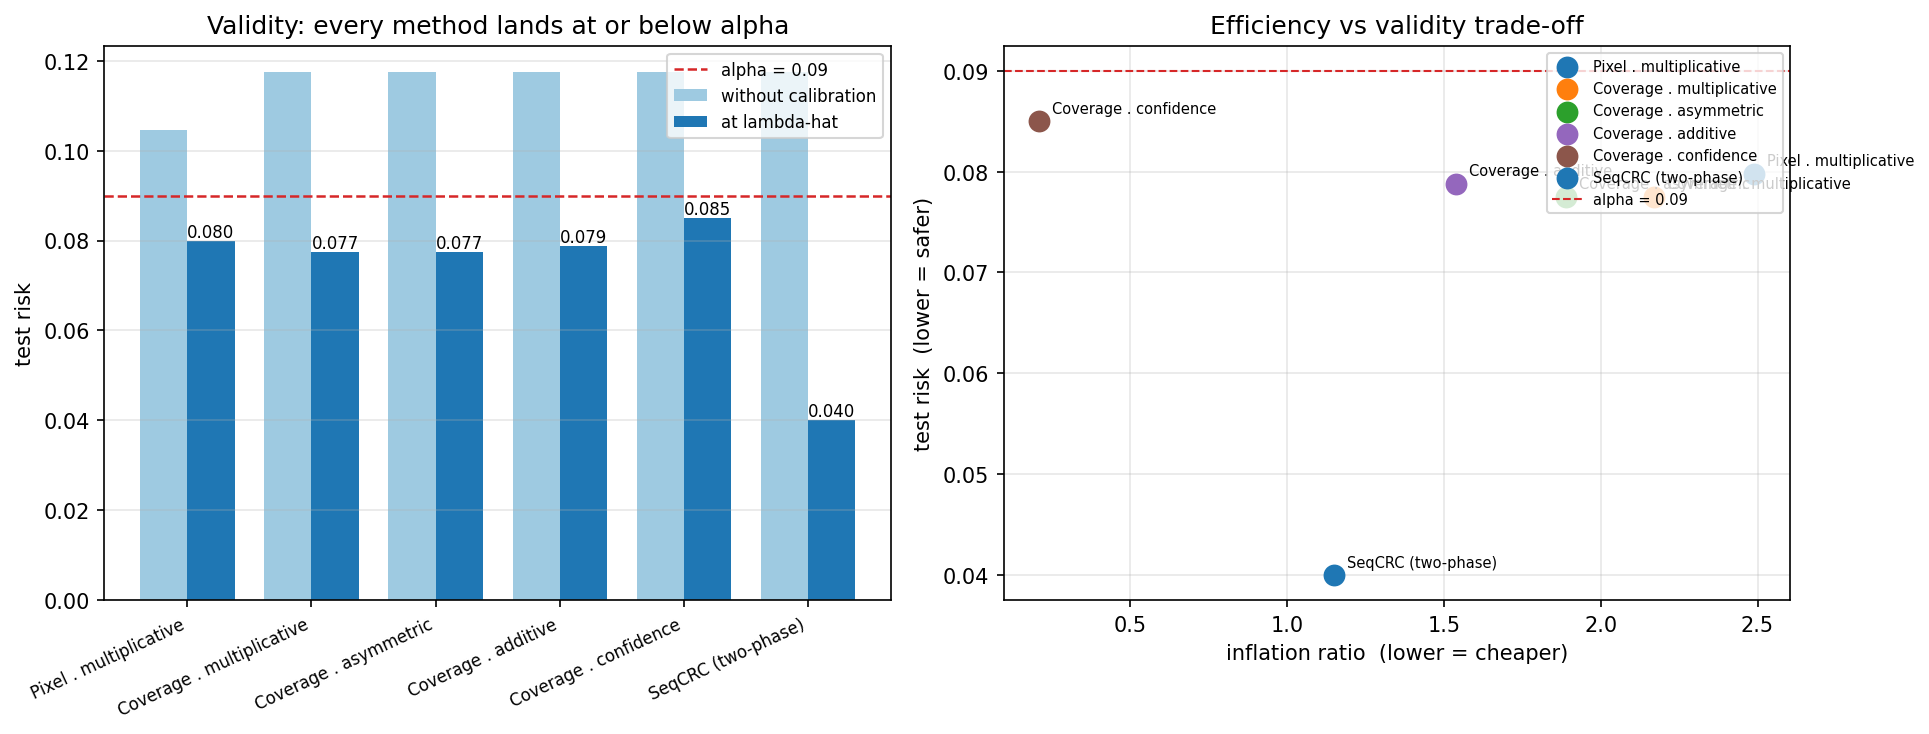
\includegraphics[width=0.98\textwidth]{fig_master_summary.png}
  \caption{\emph{Closing plot.} Left: every method's test risk vs.\ $\alpha$
  (all valid). Right: the efficiency--validity trade-off --- SeqCRC sits in the
  bottom-left (safest \emph{and} among the cheapest); the confidence knob is
  cheapest in box-count terms but leaves more clips missed.}
\end{figure}

Two failure modes of the \emph{procedure} are worth recording. First, at a
tighter $\alpha=0.085$ (\code{crc\_08}) calibration \emph{fails by design}:
$70/800$ calibration images have zero surviving predictions and lock the loss at
$1.0$, so no $\lambda$ can satisfy the bound --- a clean demonstration that
geometric expansion cannot fix a missed detection, motivating SeqCRC. Second,
the fully-missed count exposes two \emph{complementary} failure modes under the
$75\%$-coverage loss (raw detector: $94/800$ missed). The geometric single-knob
expansions enlarge boxes that already fired, cutting the count to $\sim$62/800,
but cannot help a frame where no box fired. The confidence knob does the
opposite --- it admits low-score boxes ($94\to68$/800) yet leaves them
un-enlarged, so partial-coverage frames still fall short of the $75\%$ bar.
Neither single knob dominates: each leaves the other's fixable frames missed.
Only SeqCRC composes both --- admit (Phase~1) then enlarge (Phase~2) --- and only
then does the fully-missed count fall sharply, to $32/800$.

% =====================================================================
\section{What must be done next}
% =====================================================================
\subsection{Model optimisation (the detector underneath)}
CRC certifies whatever detector it wraps; a better base detector shrinks both
$\lamhat$ and the irreducible-miss floor. Priorities:
\begin{itemize}[nosep]
  \item \textbf{Lift the miss floor.} The $\sim$62 locked frames cap every
    single-knob method. Diagnose them (\code{scripts/analyse\_motif\_errors.py},
    \code{diagnose\_top1.py}): are they tiny/occluded clips, domain-shifted
    crops, or label noise? Targeted training data there is worth more than more
    data elsewhere.
  \item \textbf{Right-size the training set.} Finish the learning-curve sweep
    (\code{docs/experiment\_plan.md}) to find $N^\star$ where mAP@.5 flattens,
    and re-calibrate at $N^\star$ --- conformal efficiency, not just mAP, should
    decide the operating point.
  \item \textbf{Confidence calibration of the detector.} The confidence knob and
    SeqCRC Phase~1 both lean on score quality; temperature/Platt scaling of YOLO
    scores could lower $T_{\text{eff}}$ for the same guarantee.
\end{itemize}

\subsection{Robustness and validity of the guarantee}
\begin{itemize}[nosep]
  \item \textbf{Exchangeability / distribution shift.} The guarantee assumes
    calibration and deployment are exchangeable. Real orthophotos differ by
    track, season, sensor. We need a shift study (calibrate on one
    track/condition, test on another) and, if shift is real,
    \emph{Mondrian / group-conditional} or weighted CRC.
  \item \textbf{Variance of $\lamhat$ and the risk.} A single $800/800$ split is
    one draw. Repeat calibration over many random splits (or
    cross-conformal/bootstrap) to report the \emph{distribution} of test risk,
    not one number, and confirm the in-expectation guarantee empirically.
  \item \textbf{SeqCRC's non-exchangeable survivor subset.} Phase~2 calibrates
    on survivors \emph{selected using the same data} (the caveat in
    \code{seqcrc.py}). The union bound is sound, but quantify how loose it is and
    whether a data-split variant tightens it.
  \item \textbf{Sensitivity to $\alpha$, the 75\% bar, and the IoU/overlap hit
    criterion} --- sweep them and report stability.
\end{itemize}

\subsection{Mathematical accuracy and methodology}
\begin{itemize}[nosep]
  \item \textbf{Monotonicity audit.} CRC's validity rests on each loss being
    monotone in $\lambda$. We argue this informally; it should be proven (or
    empirically verified to never violate) for every loss/expansion pair,
    especially the union-of-boxes pixel loss.
  \item \textbf{The Bonferroni split is loose.} The huge slack in
    \S\ref{sec:seqcrc} suggests the union bound wastes budget. Is a sharper
    multi-phase bound (or a single joint calibration) available?
  \item \textbf{Discrete-loss root finding.} Document that the CRC infimum over
    a step function is exact up to the \code{2e-6} guard, and that
    \code{brentq} is only a search convenience, not an assumption.
\end{itemize}

% =====================================================================
\section{Questions for the conformal-prediction expert}
% =====================================================================
The most leveraged questions, roughly in priority order:
\begin{enumerate}[leftmargin=1.5cm]
  \item \textbf{Validity under shift.} Our exchangeability assumption is the
    weakest link. Which tool fits geospatial rail data best --- weighted CRC,
    Mondrian/group-conditional CRC, or a covariate-shift correction --- and how
    do we estimate the shift to drive it?
  \item \textbf{Tightening SeqCRC.} Is the Bonferroni split the right way to
    compose a detection guarantee with a localisation guarantee, or is there a
    sharper sequential/joint scheme (e.g.\ a single nested loss) that avoids the
    large observed slack? How should we \emph{choose} the split
    $\alpha_{\text{cnf}}/\alpha_{\text{loc}}$ in principle rather than by sweep?
  \item \textbf{The non-exchangeable survivor subset.} Conditioning Phase~2 on
    survivors selected with the same calibration data breaks strict
    exchangeability. Is the single-set union-bound argument the accepted fix, or
    should we pay for a data split / use a leave-one-out style correction?
  \item \textbf{Loss design.} Is the per-image mean-coverage loss the right
    object, or should we control a frame-level miss indicator, an FNR/FDR-style
    risk, or use a multi-objective CRC that bounds recall and false-positive
    rate simultaneously?
  \item \textbf{Conditional rather than marginal guarantees.} Eq.~\eqref{eq:crc-guarantee}
    is marginal. Can we get a guarantee \emph{conditional} on clip size or scene
    type, given small per-group calibration counts?
  \item \textbf{Efficiency optimality.} Among monotone expansions, is there a
    principled ``most efficient'' family for thin elongated targets, or is the
    additive-vs-asymmetric comparison necessarily empirical?
  \item \textbf{Finite-sample honesty.} With $n=800$, how should we report the
    in-expectation guarantee --- is the empirical test risk plus the
    finite-sample correction enough, or do we need a PAC-style high-probability
    statement (e.g.\ via the Hoeffding/Bentkus route of conformal risk control)?
\end{enumerate}

\end{document}
